
Our previous work \cite{NOMS}, all software based, can not be deployed elsewhere than at the edge because of its limited capacity to manage more than 30Gb/s on the fly, which prevents for instance a more convenient regional deployment. To overcome this limitation, we propose to split our system into a 2-level \textit{hybrid} architecture: a data-plane programmable module to cope with high speed line-rate traffic to extract flows' features and a control-plane programmable module to perform the complex computational classification functions. For the data plane, we select P4\footnote{the P4 consortium: \url{p4.org}} \cite{P4}, which seems to be the most promising solution for data plane network programmability, and for the control plane, we rely on the NFV architecture. 

Fig. \ref{fig:chap_4:archi} depicts our architecture, with a P4-module deployed in the chipset of a hardware switch, connected to a local controller running in the Linux OS of the switch, and 3 computational modules for the detection of CG traffic. %analysis of the traffic features and the decision to classify it as cloud gaming or not.  

\begin{figure}[!t]
    \centering
    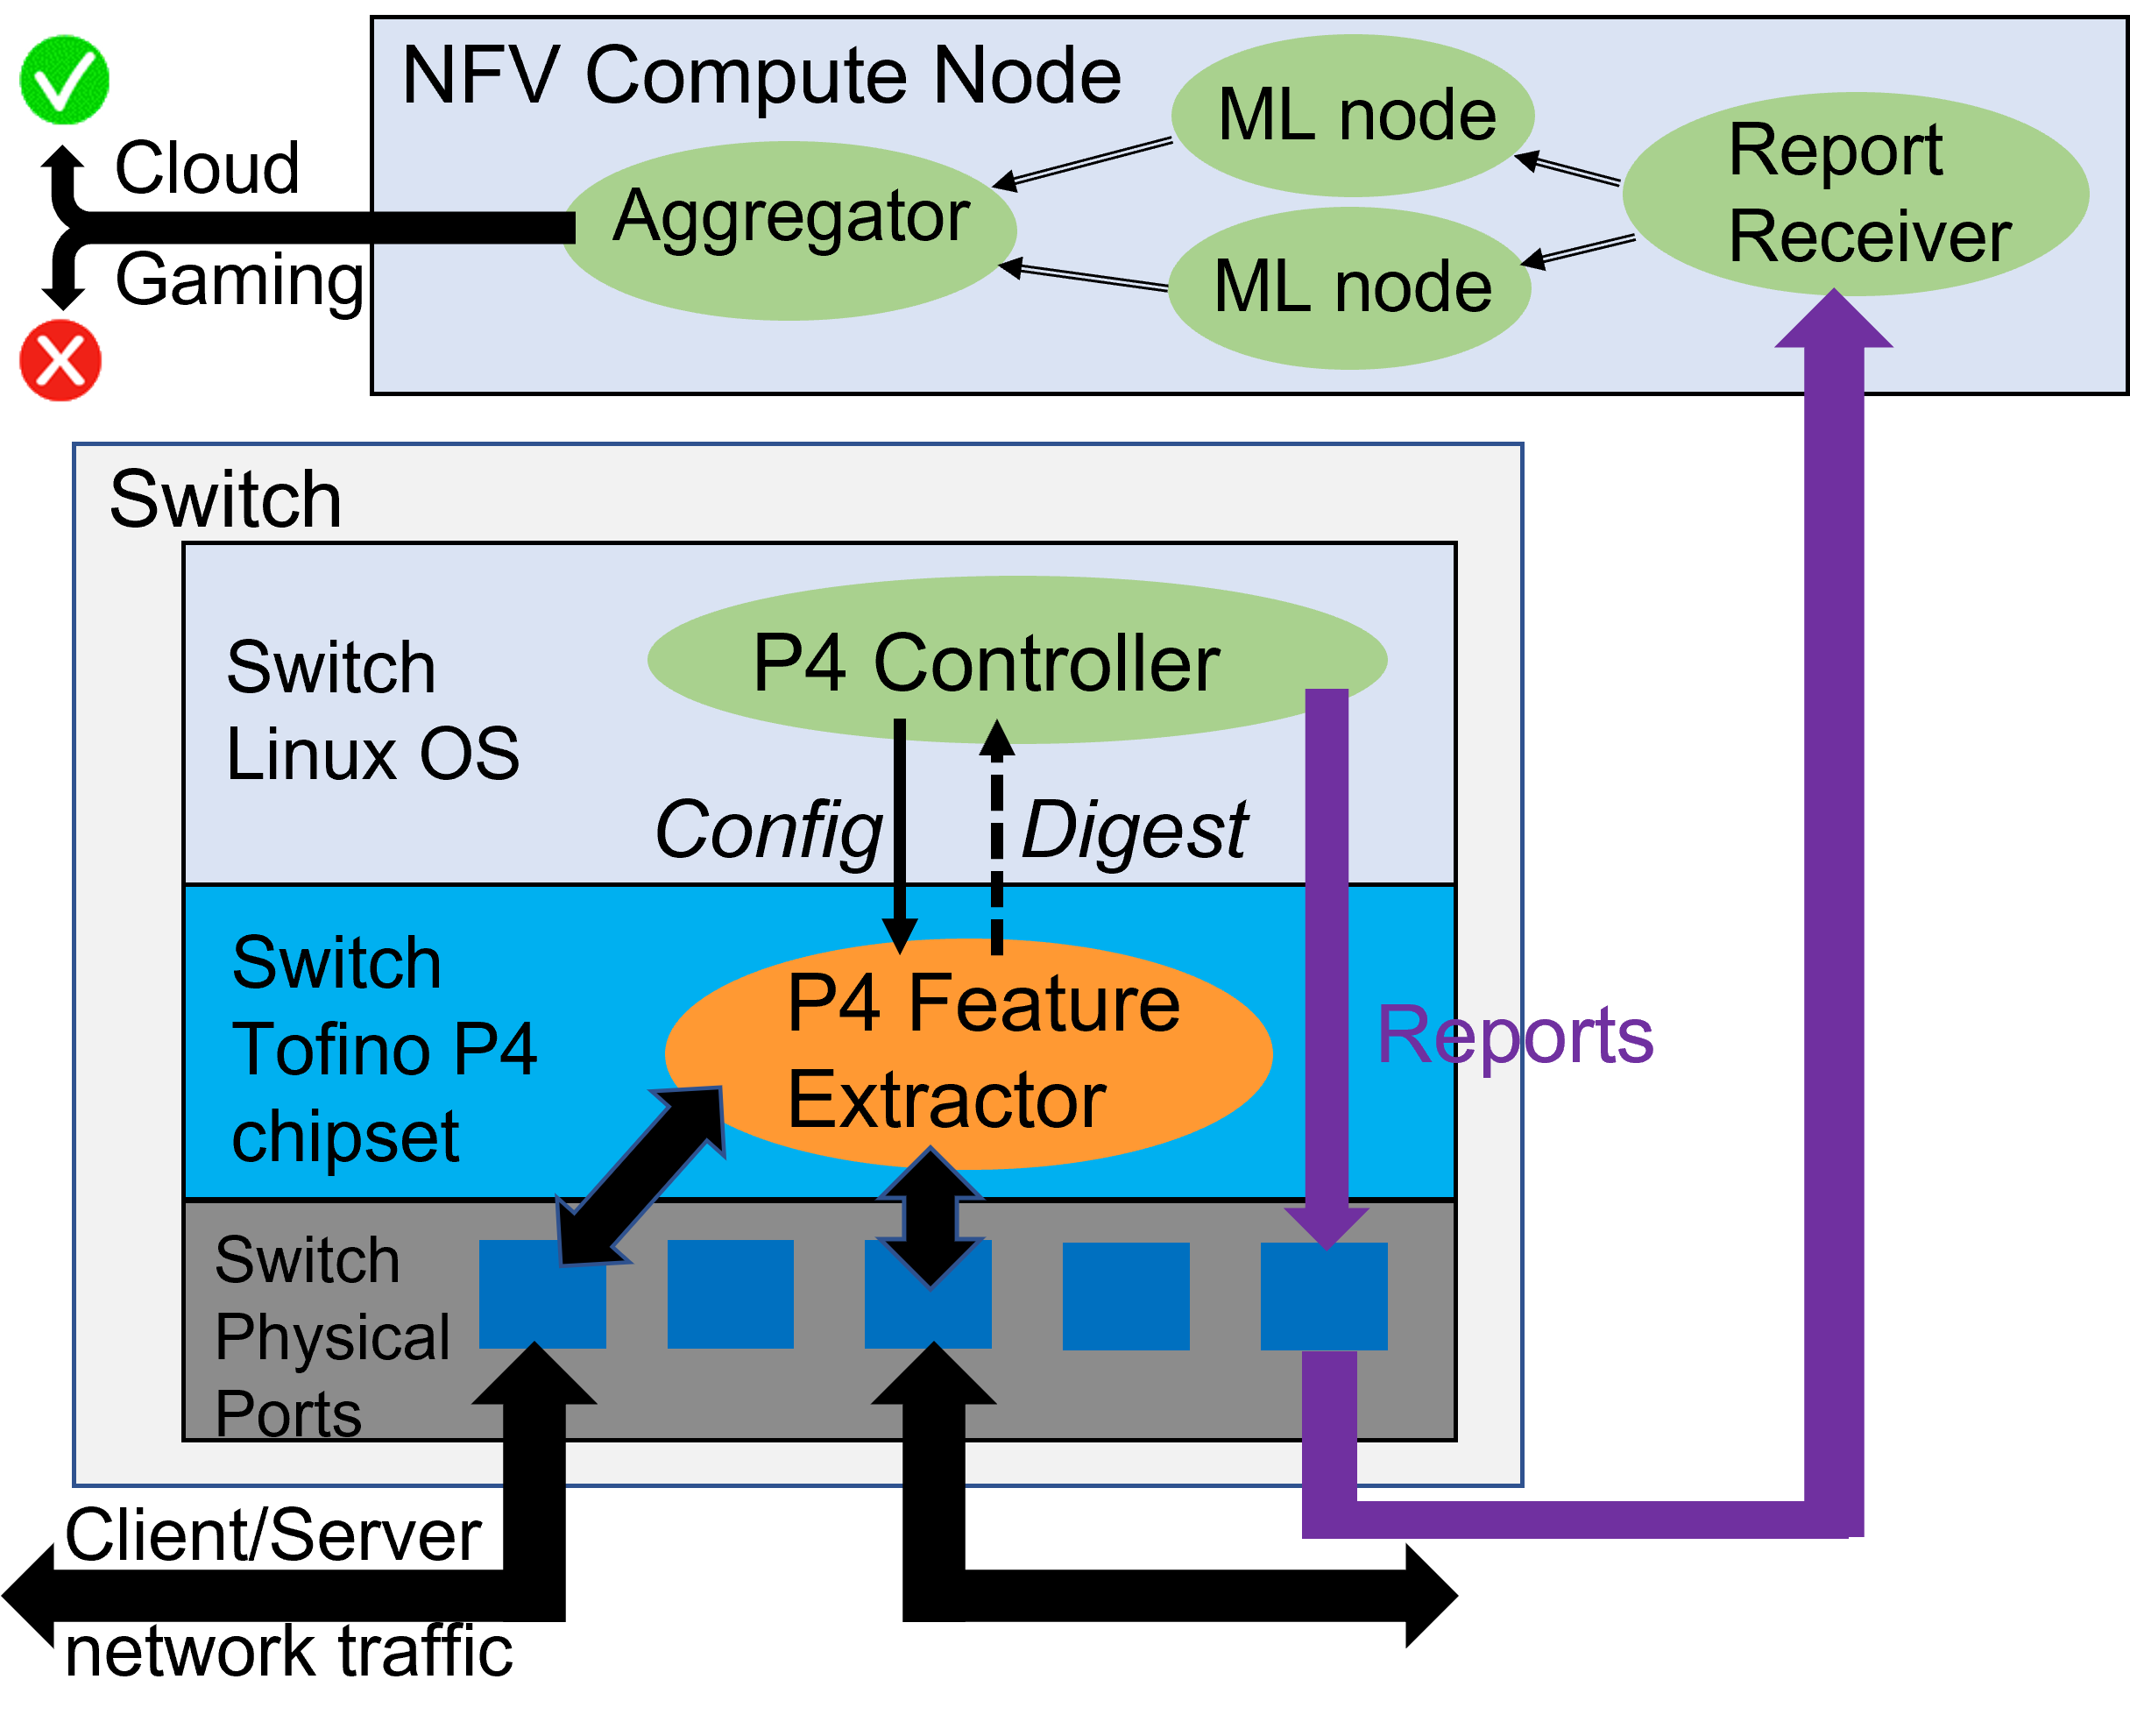
\includegraphics[width=.5\textwidth]{imgs/chapter_4/Archi_P4_NFV.png}
    \caption{The 2-level programmable architecture}
    \label{fig:chap_4:archi}
\end{figure}


\subsection{The NFV computational modules}

Although the hardware P4 module is the primary emphasis of this paper, computational VNFs are introduced below for comprehension.
%In this paper, we focus on the hardware P4 module, but for comprehension, we hereafter introduce the computational VNFs.
The complex operational tasks, mainly related to the ML processing, as described in Section \ref{chap_4:method} are developed in Python3 and run in a Linux environment in user space with all the necessary libraries (pandas, numpy, pytorch, etc.). %These VNFs are then purely user space programs.
Since the processing time is long in this environment (at least too long for line-rate processing of high speed networks), we send to them not every packet, but reports, every 33 ms, that include traffic features about the flows transiting via the P4 module during this time window. Furthermore, as presented in Section \ref{chap_4:method}, we choose a Deep Learning model USAD, which has very low inference time compared to other solutions. %\cite{}. Papier Joel ou papier USAD directement si plus complet 

In this NFV node, 3 types of VNFs are deployed: (i) one for receiving reports, extracting features values and forwarding them to the ML node, (ii) one performing the classification task, for analysing the features and giving a score indicating whether this session is cloud gaming or not, (iii) one aggregating the results from the ML nodes per flow and giving a final decision based on several time windows. In this paper, the 3 VNFs are located on the same NFV node, connected to each other via local sockets, but they can easily be deployed on different nodes if required. 

\subsection{The P4 extracting module}

To achieve a high speed line-rate processing module, we rely on the P4 approach. Since our goal is to have a realistic solution, being potentially deployed in an ISP network, we opt for a P4 hardware switch, and not the Linux-based BMv2 solution. For our testbed, we used a Edgecore Wedge 100BF-32X switch\footnote{\url{https://www.edge-core.com/productsInfo.php?cls=1&cls2=5&cls3=181&id=335}}, which is equipped with an Intel Tofino P4 chipset. This choice was primarly driven by our performance requirement of several Tb/s but has heavy implications on our work. Indeed, the P4 Tofino architecture differs from the BMv2 one and developing programs for real hardware switches presents many limitations and constraints not present in a Linux-based system (see Section \ref{chap_4:sec:limitations_P4}). This is a crucial factor to consider when compared to previous studies implementing P4 solutions using BMv2.

The Edgecore switch can be schematised with 2 levels: the low-level with the chipset responsible for line-rate packet processing and the high-level, the Linux Switch OS, in charge of the deployment, management, configuration of the chipset. In our implementation, both levels are used. Specifically, the P4 module deployed within the chipset, extracts and computes the basic packet features such as packet size and IAT. Concurrently, the Python-based controller module which runs in the Switch OS, is responsible for configuring the P4 program, receiving the reports from the P4 module (sent using the \emph{Digest} function provided by the P4 Tofino.) and transmitting the reports to the NFV node in the expected format.

\subsection{Limitations of the P4 Tofino hardware solution}
\label{chap_4:sec:limitations_P4}

In this section, we highlight the main limitations encountered when programming for a Tofino hardware switch.

%\begin{itemize}

\subsubsection{Computational limitations}

The number of operations that the P4 module in the switch can handle is limited in order to ensure a high-speed packet processing and minimize packet forwarding delays. Specifically, the Tofino 1 chipset permits a maximum number of 12 match action stages per pipeline.

Additionally, metadata in P4 are valid only for the current packet processing which requires the use of registers to save contextual information. In the hardware switch, we can have registers, but %the contents they can store is limited to maximum 32 bits or a pair of similar values of maximum 32 bits. But 
during one packet processing, only a single access to a given register is permitted. Consequently, updating a register can be done in only one step (reading the old value and writing the new one), but it is not possible to read the register, perform several other computations using the read value, and subsequently update the new computed value to the given register. This restricts and complicates the use of registers.

The Tofino P4 provides a mathematical extern unit, called \emph{MathUnit}, for complex functions like \emph{SQR} and \emph{SQRT}. However, a given register can  have only a single \emph{MathUnit} extern, and RegisterActions sharing a register can only use one MathUnit between them. Consequently, it is not possible to compute \emph{SQR} and \emph{SQRT} for the same value during the processing of one packet, thereby making the computation of the standard deviation impossible.  
%Finally we tried, a much more simplification with an alternative computation in our first version of the P4 Extractor module. And even with this processing optimisation/limitation, we reached the 12 stages for one packet processing. 

\subsubsection{Computation limited to the current packet}
The computation of the standard deviation feature poses another challenge. Since its computation is based on the mean value, we need to store in the memory all the packets within a time window and compute the mean and standard deviation at the end of the time window. However, the P4 Tofino hardware switch lacks a packet buffering/copying capability. To address this limitation, we explored the Welford's algorithm to compute the standard deviation online but the P4 Tofino hardware switch does not support variable multiplication and division. Consequently, we attempted to approximate the standard deviation through a simple computation. However, as depicted in Fig. \ref{fig:chap_4:result_variance_P4}, this approximation adversely affected the classification performance compared to the accurate computation of the standard deviation.

\begin{comment}
There is another issue with the computation of the standard deviation. Indeed it is computed based on the mean value of the feature for all the packets in the time window (33 ms in our case).  We then have to keep in memory (eg. done with a list or a dictionary with a programming language) all the packets of the time window, wait for the end of the window to compute the mean value and then compute the standard deviation of all packets. However, the P4 Tofino hardware switch does not provide such a packet buffering/copying capability. We investigated the implementation of the Welford's algorithm, making possible to compute the variance in one pass, but we faced computational limitations, being not possible to multiply and divide with variable values. Finally, we tried to overcome this limitation by approximating a simple computation for the standard deviation, however, our evaluation given in Fig. \ref{fig:chap_4:result_variance_P4} reveals that this approximation harms the classification performance compared to the correct computation of this feature. 
\end{comment}
%Examining the results of each platform, we found that the performance was good for PSN and XC, but poor for GFN and STD, whose behaviour is more dynamic and thus the standard deviation feature has a great importance in the ML model decision.
%role (taken into consideration by the ML model).   

\begin{figure}[!t]
    \centering
    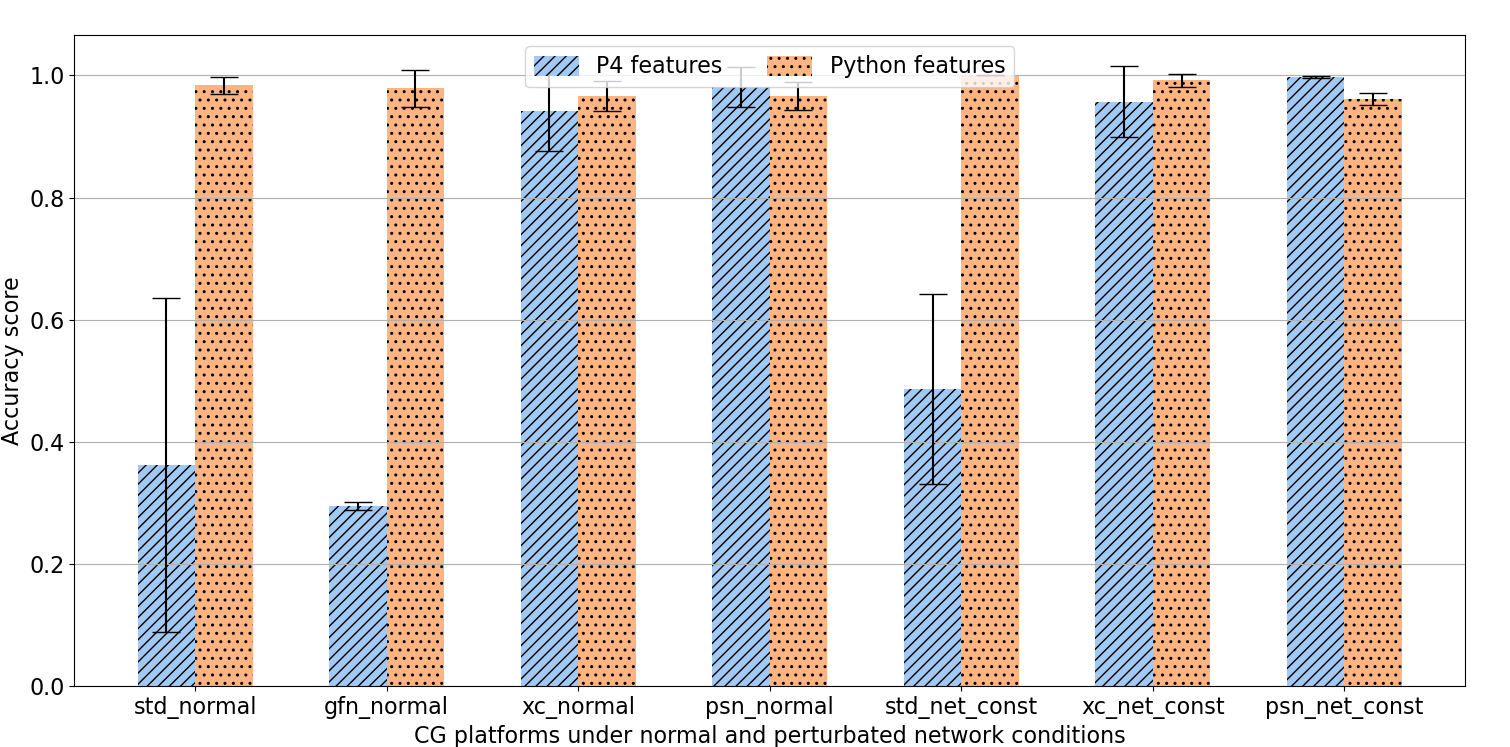
\includegraphics[width=.8\textwidth]{imgs/chapter_4/comparison_p4_python.png}
    \caption{Performance of the ML model with the standard deviation with P4-extracted features}
    \label{fig:chap_4:result_variance_P4}
\end{figure}

In light of these challenges, we decided to train the ML model without the two standard deviation features. Surprisingly, the simplified model exhibited strong performance and achieved results similar to the model with standard deviation, as illustrated in Fig.\ref{fig:chap_4:result_variance_or_not}. Removing the standard deviation features in the P4 extracting module then greatly simplifies the program and its P4 processing (only 6 stages are now necessary to process the packet). Moreover, the notable efficiency of this approach prompts us to retain this novel approach.

% BM : A faire figure plus tard
\begin{figure}[!t]
    \centering
    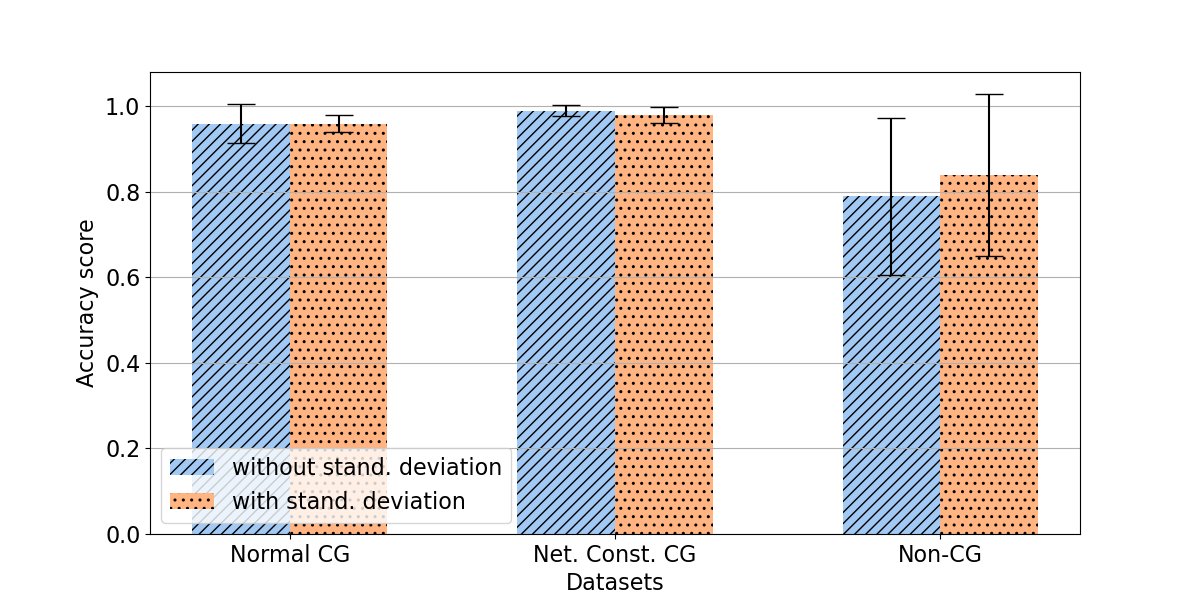
\includegraphics[width=.8\textwidth]{imgs/chapter_4/variance_impact.png}
    \caption{Performance of the ML model with and without the standard deviation}
    \label{fig:chap_4:result_variance_or_not}
\end{figure}




\subsubsection{Size of \emph{Digest} message}

As mentioned in the beginning of this section, we use the \emph{Digest} mechanism to send reports from the P4 module to the controller. However, the Tofino hardware restrics the size of the \emph{Digest} message to 48 bytes. In our previous version with the standard deviation, we reached this maximum value when sending all the 12 features and had no space left to send the couple of IP addresses identifying the flow. Without the four standard deviation features (for the packet size and the IAT in both directions), we have now enough space to include the IP addresses and port numbers.

\subsubsection{Limited time-based processing}

In the design of our ML model, we use time windows of 33 ms to split the session data in order to compute the features. This can be easily done with an application programming language such as Python or C++ using time handler, but not with P4. Indeed, a P4 program can trigger actions upon the reception of one packet, but not at a given time. Even if the Tofino offers the possibility to generate packets at a periodic interval, it is not suitable for our case. Indeed, the payload of the generated packet is set up by the configuration plane and even if modifying this payload is possible in the P4 program, we can not make it for all the sessions passing through the switch.  Therefore, we opt for the \emph{Digest} approach and manage this timing inside the P4 program by using one register to store the time when a first packet arrives and at each packet arrival, we check whether the time exceeds the required time window  of 33 ms. If so, we send the report to the controller. It means that for regular and high bitrate sessions, for which we can expect very frequent packet arrivals, this way of computing the time window can be close to the 33 ms time, but
for low-rate traffic, sporadic or bursty traffic, this approach is not appropriate because of possible long time intervals between packet arrivals. %(and then triggers the end of the window computations and the sending of the report).
For NCG traffic, this limitation greatly degrades the performance of our solution since very few reports are sent over long periods, being non representative of the application traffic  behavior. To circumvent it, we include a time handler in our controller module which generate \emph{empty} reports and send them to the NFV compute node if the time interval between the reception of two reports is longer than two time windows of 33 ms. As such, the ML module can have reports, close to what it expects (i.e. a regular 33 ms basis). Despite being a major improvement, this solution is still not perfect since for example, if one packet arrives at $t+31$ ms and the next one at $t+46$ ms, the report sent by the P4 module will be related to a 46ms time window and not a 33ms one. Consequently, the ML model will not be aware that there was no traffic during the missing 13ms.

%\end{itemize}

In conclusion, we have learned several lessons based on our experience with P4 implementation on a real hardware switch. Firstly, the P4 program cannot not perform many processing tasks for a single packet, cannot handle complex computational tasks and is not really suitable for programs with time based events. Therefore, careful consideration and optimization are required when developing a P4 code.

Secondly, a trade-off must be made between the high speed line-rate packet processing and the ease of programming, as well as the complexity of the computational tasks. Our proposed  2-level programmable architecture appears to be a promising approach to meet both factors, the developers splitting the processing adequately.
